\chapter{电路设计与仿真}

本章对基于Cadence Virtuoso仿真软件和SMIC 0.18um BCD工艺设计的变换器芯片的各个关键电路进行分析和仿真,包括欠压锁定电路、内部供电电路、模式切换电路、退磁时间动态校准电路、峰值电流控制电路、精确谷底导通电路、谷值锁定电路、逻辑控制电路和各个保护电路等。最后对整体电路进行系统仿真,测试变换器芯片的基本功能,验证该电路设计的合理性和可靠性。

\section{欠压锁定电路}




\section{内部供电电路}

\subsection{带隙基准电路}

在变换器芯片工作过程中,其内部的各个模块都需要相应的偏置电压和偏置电流,为了维持这些偏置电压和偏置电流的精确和稳定性,不能用普通的与电源无关的基准电路产生全部的信号,因此需要设计带隙基准电路,提供受电源电压和温度变化影响很小的基准电压电流,使得变换器芯片适用于各种工况下。

带隙基准电路的实现原理是通过将一个正温度系数的电压和一个负温度系数的电压加权相加后,抵消掉其正负温度系数,得到不受温度变化影响的零温度系数的基准电压。实际电路中,负温度系数的电压利用双极型晶体管产生,其正向压降$V_{be}$带有负温度特性。通过半导体物理的基础知识可知,电压$V_{be}$的公式为:
\begin{equation}
    \label{eq:Vbe公式}
    V_{be} = V_T \cdot ln(\frac{I_c}{I_s})
\end{equation}
其中,$V_T$是热电压,公式为:
\begin{equation}
    \label{eq:VT公式}
    V_T=\frac{kT}{q}
\end{equation}
$I_c$是PN结的集电极电流,公式为:
\begin{equation}
    \label{eq:Ic公式}
    I_c=I_s \cdot exp(\frac{V_{be}}{V_T})
\end{equation}
$I_s$是PN结饱和电流,公式为:
\begin{equation}
    \label{eq:Is公式}
    I_s=bT^{4+m} exp\frac{-E_g}{kT}
\end{equation}
结合式\eqref{eq:Vbe公式}、\eqref{eq:Ic公式}和\eqref{eq:Is公式},通过正向压降$V_{be}$对温度求偏导,可计算得$V_{be}$的负温度系数公式:
\begin{equation}
    \label{eq:Vbe/T公式}
    \frac{\partial V_{be}}{\partial T} = \frac{ V_{be} - (4+m)V_T - E_g/q}{T}
\end{equation}

正温度系数的电压同样可以通过双极型晶体管来产生,不同电流密度的电流流经晶体管会产生不同的负温度系数,两者的差值电压$\varDelta V_{be}$带有正温度系数。实际电路中为了满足晶体管的匹配性,使用两个不同面积的双极型晶体管来产生不同电流密度的作用。令两个双极型晶体管的面积比为$1:N$,则流经单个晶体管的电流密度比N:1,可计算得晶体管压差$\varDelta V_{be}$的公式为:
\begin{equation}
    \label{eq:△Vbe公式}
    \varDelta V_{be} = V_T ln(\frac{I_c}{I_s}) - V_T ln(\frac{I_c}{nI_s}) = V_T \cdot ln(n)
\end{equation}
通过$\varDelta V_{be}$对温度求偏导可计算得正的温度系数公式:
\begin{equation}
    \label{eq:△Vbe/T公式}
    \frac{\partial \varDelta V_{be}}{\partial T} = \frac{k}{q}\cdot ln(n)
\end{equation}


由式\eqref{eq:Vbe/T公式}和\eqref{eq:△Vbe/T公式}计算可知,在常温T=300K的条件下,当$V_{be}\thickapprox $ 750 mV时,$V_{be}$的负温度系数约等于-1.5 mV/K,$\varDelta V_{be}$的正温度系数为0.087ln(n) mV/K。为了合理地产生零温度系数电压,防止双极型晶体管的面积太大,需对正负温度系数加权相加可得。

为了满足变换器芯片中的低压数字模块,



\subsection{高压LDO电路}

由辅助绕组产生的供电端电压对于片内的元器件而已电压过大且不够稳定,无法直接用于作为供电电压,需要设计用于产生稳定输出电压的低压线性稳压器电路,将供电端的高压转化为可为内部电路供电的电源电压输出。
\begin{figure}[htbp] 
    \centering
    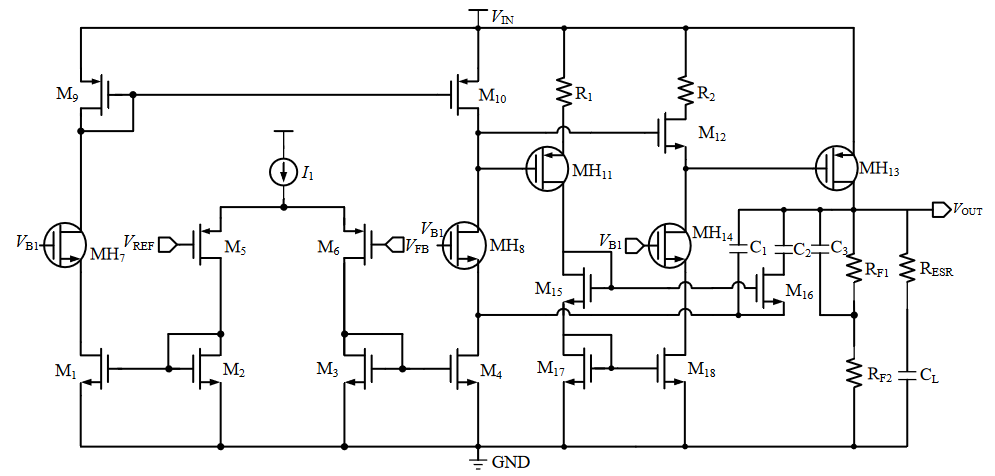
\includegraphics[width=0.6\linewidth]{figures/高压LDO.png}
    \caption{高压LDO电路图}
    \label{fig:高压LDO}
\end{figure}

本文设计的高压LDO电路如图~\ref{fig:高压LDO}所示,该电路


%\section{抖频振荡器}

\section{模式切换电路}

\section{退磁时间动态校准电路}

\section{峰值电流控制电路}

%\section{前沿消隐电路}

\section{精确谷底导通电路}

根据上文3.6.2节介绍的精确谷底导通技术,本小节对图~\ref{fig:精确谷底导通技术框图}中的精确谷底导通模块进行具体的描述并仿真其基本功能。

图~\ref{fig:精确谷底导通电路图1}是精确谷底导通模块的电路框图。包括两个峰值检测电路、压控高通滤波器、SR锁存器、鉴相鉴频器、电荷泵和逻辑电路等。

\begin{figure}[htbp] 
    \centering
    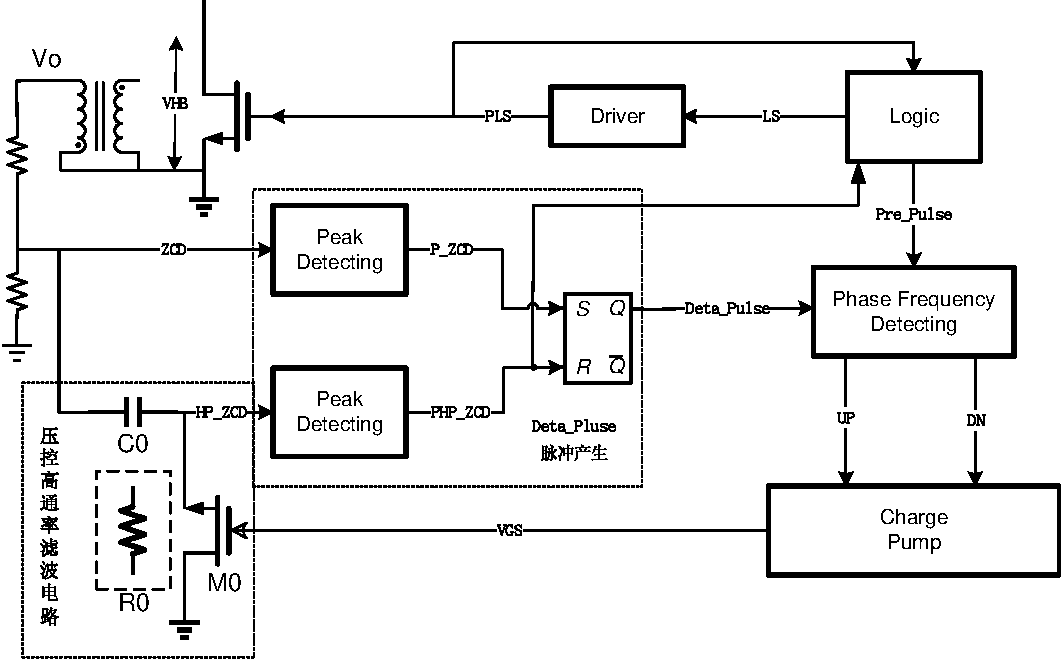
\includegraphics[width=0.8\linewidth]{figures/精确谷底导通电路图1.pdf}
    \caption{精确谷底导通电路图1}
    \label{fig:精确谷底导通电路图1}
\end{figure}


因为功率管半桥节点信号$V_{HB}$的电压值过大,因此对在等待时间内同样带有谐振信息的辅助绕组分压引脚ZCD的电压信号$V_{ZCD}$进行采样处理。由于$V_{ZCD}$信号和$V_{HB}$信号的谐振电压相位相反,故$V_{HB}$的谐振谷底对应$V_{ZCD}$的谐振谷峰值。如图~\ref{fig:精确谷底导通电路图1}中所示,采用峰值检测电路来检测$V_{ZCD}$信号在等待时间$T_w$内的谐振谷峰值,并输出对应的峰值脉冲信号。

峰值检测电路图如图~\ref{fig:峰值检测电路图}所示。峰值检测电路包括一个由晶体管M2、M4、M5、M6和M7组成的五管运算放大器,一个晶体管M9和M10组成的电流镜以及一个M11构成的源极跟随器。电流源M12为源极跟随器M11提供偏置电流。该电路的工作原理是通过运算放大器比较输入电压$V_{in}$和输出电压$V_{out}$的大小,当输入电压$V_{in}$大于输出电压$V_{out}$时,运算放大器输出低电平,拉低电流镜晶体管M9的栅端电压,电流镜开始工作,对电容$C_1$进行充电,电压$V_1$逐渐升高,$V_{out}$在源极跟随器的作用下也逐渐增大,跟随$V_{in}$。当$V_{in}$不再增大,$V_{in}$开始小于$V_{out}$时,运算放大器输出高电平,电流镜晶体管M9的栅端电压被拉高,电流镜停止工作,不再给电容$C_1$进行充电,进而输出电压$V_{out}$也保持不变,实现峰值检测的目的。最后通过一个脉冲产生电路输出脉冲信号P\_ZCD。同时为了检测在电路在不同周期内不同大小的输入电压$V_{in}$,加入复位开关晶体管M13,当接收到复位信号后,M13导通,对V1进行放电,实现复位的功能。

\begin{figure}[htbp] 
    \centering
    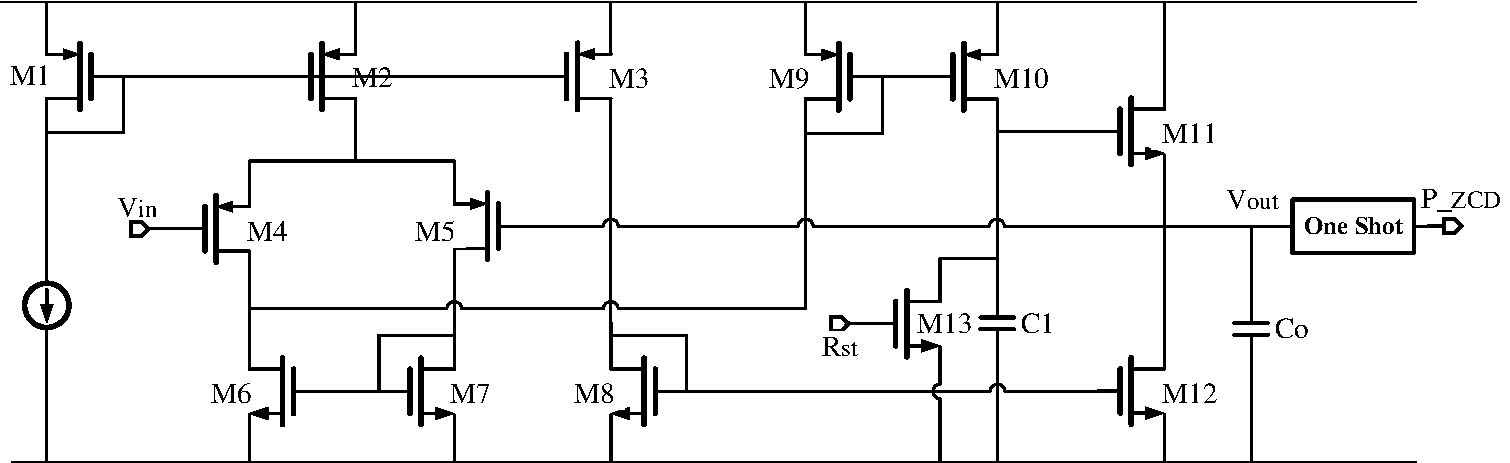
\includegraphics[width=0.8\linewidth]{figures/峰值检测电路图.pdf}
    \caption{峰值检测电路图}
    \label{fig:峰值检测电路图}
\end{figure}

由于驱动电路等电路结构对逻辑控制信号存在延时问题,为了满足精确的谷底导通功能,不能直接将峰值检测电路产生的峰值脉冲信号P\_ZCD直接作为时钟信号CLK输入到逻辑控制模块,产生下个开关周期的逻辑控制信号LS。针对于该问题,需要在$V_{HB}$谐振谷底到达之前产生低边功率管的导通时钟信号,使得逻辑控制信号LS通过驱动电路后,输出的栅极驱动信号LSGD恰好位于$V_{HB}$信号谐振谷底的位置处,此时导通低边功率管,不仅降低开关损耗,还极大地减小峰值检测电压的过冲现象。因此要求逻辑控制信号LS超前产生的时间近似等于驱动电路等的延时时间。

该模块中实现超前采样$V_{ZCD}$信号峰值的核心电路是采用的压控高通滤波器电路,如图~\ref{fig:精确谷底导通电路图1}中所示,可以通过控制MOS管的栅极电压$V_{GS}$来调节MOS管的导通电阻$R_{on}$,$R_{on}$的计算公式为:
\begin{equation}
    \label{eq:Ron公式}
    R_{on}=\frac{1}{\mu_n C_{ox} \frac{W}{L} (V_{GS} - V_{TH})}
\end{equation}
由式可知,随着MOS管栅极电压$V_{GS}$的增大,其导通电阻逐渐减小。根据高通滤波器的幅频曲线公式可知,当功率管栅压$V_{GS}$为零电压时,功率管截止,导通电阻近似无穷大,对应的时间常数RC无穷大,相位变化为0度,压控高通滤波器的输出信号$V_{ZCD,PH}$和信号$V_{ZCD}$的电压波形重合。随着栅压信号$V_{GS}$的增大,时间RC常数越小,$V_{ZCD,PH}$波形超前的相位变化越大,直至时间常数RC等于零时,超前相位最大值90度。
\begin{equation}
    \label{eq:jw公式}
    \varphi_{j\omega }=\arctan (\frac{\omega_c}{j\omega R C })
\end{equation}
其中$\omega_c$为滤波器的截止频率。通过和合理的调节MOS管栅压信号$V_{GS}$的值,即可调节$V_{ZCD,ph}$波形恰好超前$V_{ZCD}$电压波形的相位时间等于驱动电路的延时时间,实现低边功率管栅极驱动信号的精确谷底导通功能。

如图~\ref{fig:精确谷底导通电路图1}中所示,压控高通滤波器的栅压信号$V_{GS}$的调控方式采用了锁相环电路中的鉴相鉴频器和电荷泵结构来动态调节实现。图~\ref{fig:鉴相鉴频器电路图}为该模块使用的鉴相鉴频器电路和电荷泵的电路图。包括两个带复位端的下降沿D触发器和一个与门组成。触发器的D输入端都接高电平保持逻辑"1",触发器1的时钟输入端D\_Phase是信号$V_{ZCD,PH}$和信号$V_{ZCD}$波形的超前相位时间差;触发器2的时钟输入端L\_Phase是逻辑控制信号LS和栅压驱动信号LSGD的延迟时间差。通过这两个D触发器检测D\_Phase和L\_Phase信号的相位时间差信号UP和DN,再通过信号UP和DN控制电荷泵的开关S1和S2,选择对电容$C_{GS}$进行充电或放电功能。

\begin{figure}[htbp] 
    \centering
    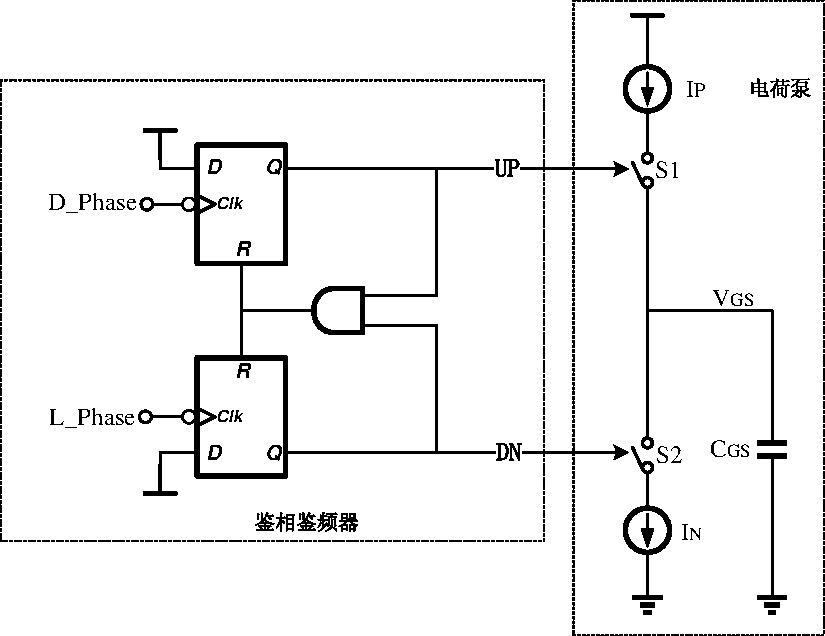
\includegraphics[width=0.6\linewidth]{figures/鉴相鉴频器.pdf}
    \caption{鉴相鉴频器和电荷泵电路图}
    \label{fig:鉴相鉴频器电路图}
\end{figure}

鉴相鉴频器和电荷的波形图如~\ref{fig:鉴相鉴频器波形图}所示。不同于上升沿D触发器组成的鉴相鉴频器,该模块中使用的下降沿鉴相鉴频器的输出信号UP和DN是信号D\_Phase和L\_Phase的下降沿的相位时间差。当信号D\_Phase先于信号L\_Phase变为低电平时,信号UP由低变高,导通开关S1,电流源$I_P$对电容$C_{GS}$进行充电,电压$V_{GS}$逐渐增大;当信号L\_Phase的下降沿到来后,UP由高变低,开关S1关断,$V_{GS}$保持不变。同理,信号DW和UP相似,区别在于L\_Phase先于信号D\_Phase变为低电平时有低变高,导通开关S2通过电流源$I_N$对电容$C_{GS}$进行放电,电压$V_{GS}$逐渐减小。随着鉴相鉴频器和电荷泵电路的不断工作,最终信号D\_Phase和信号L\_Phase几乎重叠,信号UP和DN脉冲保持一致,同时给电容$C_{GS}$进行充电和放电,电压$V_{GS}$维持稳定。

\begin{figure}[htbp] 
    \centering
    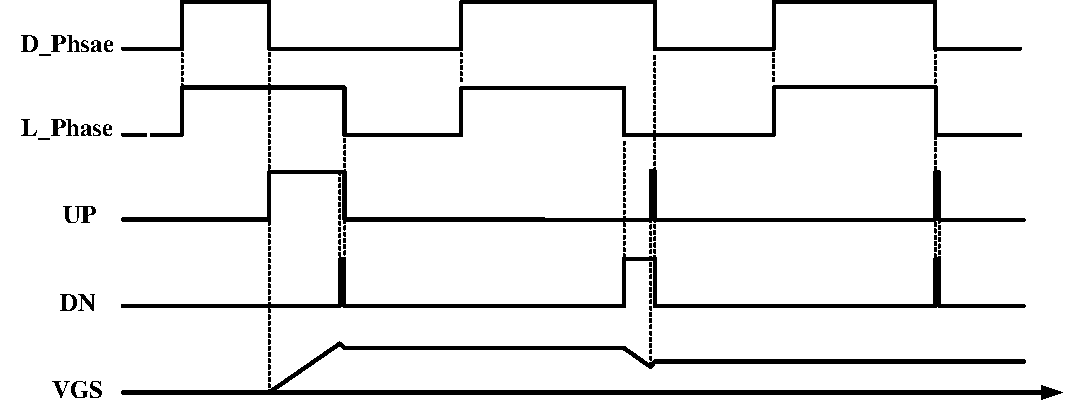
\includegraphics[width=0.8\linewidth]{figures/鉴相鉴频器波形图.pdf}
    \caption{鉴相鉴频器电荷泵波形图}
    \label{fig:鉴相鉴频器波形图}
\end{figure}

%通过逻辑控制电路得到LS和PLS信号的延时时间Pre\_Pulse。为了预判谷底信号,通过一个使用MOS管充当电阻的压控高通滤波器电路,产生$V_{ZCD}$对应的超前时间信号VHP\_ZCD,只需适当的调节VGS的大小即可控制VHP\_ZCD信号的超前时间大小。分别使用两个峰值检测电路来检测并得到两个信号的峰值脉冲信号,经过SR锁存器产生超前时间Deta\_Pulse。为了轻微的调节栅极电压信号VGS,使用了PLL电路中的鉴相鉴频器和电荷泵电路来控制Deta\_Pulse信号逐步逼近Pre\_Pulse信号,完成低边功率管的精确谷底导通功能。


\section{谷值锁定电路}

\section{逻辑控制电路}

\section{保护电路}

\section{系统整体仿真}

\section{小结}




